\documentclass[12pt]{article}

\textheight     = 220mm
\textwidth      = 160mm
\topmargin      =  -5mm
\oddsidemargin  =   2mm
\evensidemargin =   2mm

\usepackage{alltt}
\usepackage{amsfonts}
\usepackage{amsmath}
\usepackage{amssymb}
\usepackage{bm}
\usepackage{boxedminipage}
\usepackage{color}
\usepackage{float}
\usepackage{framed}
\usepackage{glossaries}
\usepackage{graphicx}
\usepackage{hyperref}
\usepackage{subfigure}

\hypersetup
{
    bookmarks=true,         % show bookmarks bar?
    unicode=false,          % non-Latin characters in Acrobat’s bookmarks
    pdftoolbar=true,        % show Acrobat’s toolbar?
    pdfmenubar=true,        % show Acrobat’s menu?
    pdffitwindow=false,     % window fit to page when opened
    pdfstartview={FitH},    % fits the width of the page to the window
    pdftitle={My title},    % title
    pdfauthor={Author},     % author
    pdfsubject={Subject},   % subject of the document
    pdfcreator={Creator},   % creator of the document
    pdfproducer={Producer}, % producer of the document
    pdfkeywords={keyword1} {key2} {key3}, % list of keywords
    pdfnewwindow=true,      % links in new window
    colorlinks=true,       % false: boxed links; true: colored links
    linkcolor=black,          % color of internal links (change box color with linkbordercolor)
    citecolor=black,        % color of links to bibliography
    filecolor=black,      % color of file links
    % linkbordercolor=black,
    urlcolor=black           % color of external links
}

\begin{document}

\begin{center}
    \Large{Coursera Capstone - A Comparison of a Suburb's Median House Price in Four Major Australian Cities}\\
    \vspace{5pt}
    \large{Stephen Moore}
\end{center}

\section{Introduction}

    In this assignment we will study the median house prices in the different suburbs of four major Australian cities, namely Brisbane, Melbourne, Sydney, and Perth. The goal will be to investigate the relatively simple questions of whether the median house price correlates with the distance to the central business district (CBD), or whether it can be better correlated to the types of venues that are found within the suburb. Furthermore, the differences in prices and will be compared between the four cities. The value for such an analysis could be realised by any business involved in real-estate where a detailed knowledge of house prices in different cities and suburbs could add value to potential clients. One particular example could be in an online tool recommending different suburbs in different cities to people interested in immigrating to Australia, based on the financial situation, for example. Furthermore, the analysis could be used to provide information about the types and prevalence of different venues within a suburb of interest.

\section{Data}

    % Suburb profile website screenshot
    \begin{figure}[h!]
        \begin{center}
            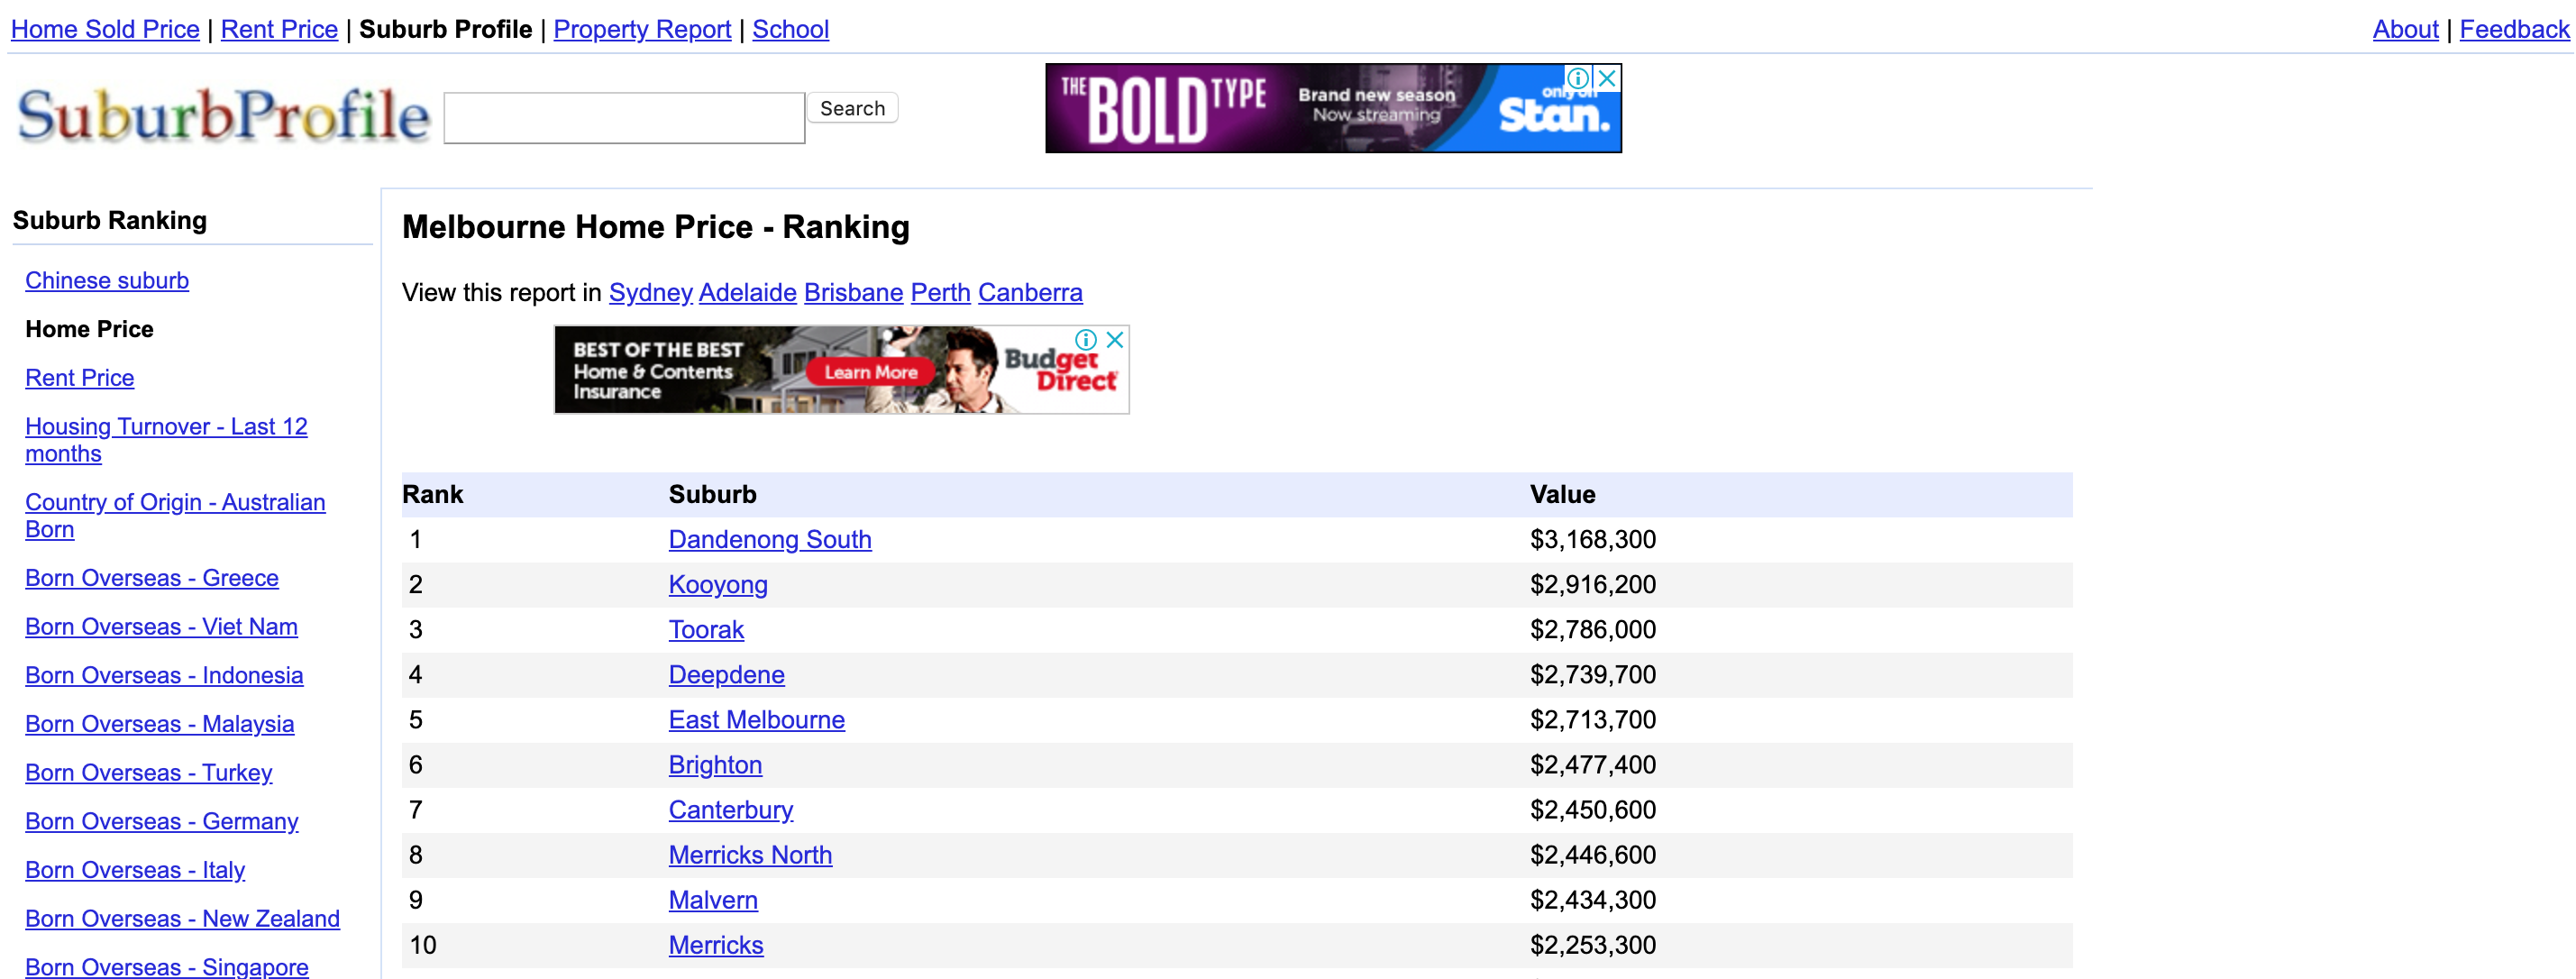
\includegraphics[width=0.9\textwidth,keepaspectratio]{Figures/SuburbProfileScreenShot}
            \caption{Screenshot of the \href{http://house.speakingsame.com/suburbtop.php?sta=qld&cat=HomePrice&name=&page=0}{Suburb Profile website}.}
            \label{Fig:SuburbProfileScreenShot}
        \end{center}
    \end{figure}

    The primary data source for this assignment is the `Suburb Profile' website, that contains tables of median house prices for the different suburbs, as depicted in Figure \ref{Fig:SuburbProfileScreenShot}. This data will be scraped and assembled into a data frame using the \emph{Beautiful Soup} library. In addition, the geographic coordinates of the city CBD and suburbs will be gathered via the \emph{Nominatum} geocoder API and the categories of nearby venues in each suburb will be gathered via the \emph{Foursquare} API.

\section{Methodology}

    In order to assemble the initial data frame from the Suburb Profile website it is important to note that only fifty suburbs are listed per page, with a `next' link to manually move from page to page. In order to automate the process of web scraping process an entity `\texttt{\&page=0}' is appended to the URL such that the HTML can be requested inside a for loop, incrementing the page counter. As can be observed in Figure \ref{Fig:SuburbProfileScreenShot}, the data is contained in a table, which can be easily found with Beautiful Soup by finding all table rows (with the \texttt{tr} tag). Within these rows a regular expression can be used to find standard table cells (with the \texttt{td} tag) that have a dollar sign in them, followed by a number. The suburb and price can then be obtained by getting the first and second siblings of the table row.

    Having compiled the suburbs and prices for each city, the next step is to find the latitude and longitude for each suburb. The most efficient way to achieve this for a large number of locations is to use the `RateLimiter' function from the geopy library, passing it the data frame of suburb names. As a side note, it was observed that in order to successfully locate the suburbs in their respective cities, search terms that concatenate the suburb name with the city, state, and country names were added to the data frame so that, for example, Nominatum wouldn't return locations in Europe or North America in the cases where suburbs with the same names exist there. Once the geographic coordinates of each suburb were found, the distance to the CBD was computed using the `distance' function from the geopy library. This function takes as input two sets of (lat,lon) coordinates and can output a distance in kilometers. To limit the number of suburbs to those which could reasonably be considered part of the city a cutoff value of 40km was used to which any suburb farther from the CBD was dropped from the resulting data frame.

    The final step in compiling the dataset involved getting nearby venues within each suburb. Using the Foursquare API to explore each suburb location with radius of 1km and limiting the search to 100 results another data frame was created for each city.

    The subsequent analysis involved initially visualising the distributions of house prices for the four cities and then creating Leaflet maps to visualise the house prices within each suburb. Using the nearby venues data frames, some simple k-means clustering was performed for each city using the `Elbow method' to determine the most appropriate number of clusters and then creating Leaflet maps to display the clusters, such that a visual comparison to the house prices can be made.

    Using the distance to the CBD as a simple metric a simple polynomial regression analysis was performed for each city, exploring how reasonable the notion of using just the distance to the CBD as a single feature in predicting a suburbs' median house is. Following this analysis a simple regression was performed using a support vector regressor (SVR) instead using one-hot encoded venue categories, in order to explore whether there is any utility in attempting to use the types of venues found within a suburb to predict its median house price. While intuitively one would not necessarily think that this would be an effective way to predict house price, a large parameter sweep using the \texttt{GridSearchCV} function was performed in order to determine the best possible hyper-parameters with which to make the prediction.

    % describe prices site and web scraping
    %     site format td with dollar sign
    %     creating full name with geocoder
    %     distance with nominatum
    % describe venues
    % describe clustering
    %     elbow method to find optimal num clusters
    % describe regression
    %     grid search for hyperparameter tuning, cross validation

\section{Results}

    % Suburb price distribution for all cities
    \begin{figure}[h!]
        \begin{center}
            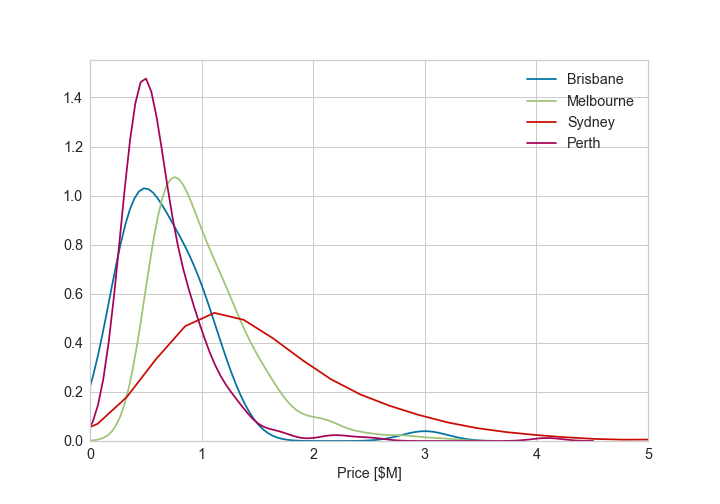
\includegraphics[width=0.75\textwidth,keepaspectratio]{Figures/SuburbPriceDistributionsForAllCities}
            \caption{Distributions of house prices in the different suburbs of the four cities considered.}
            \label{Fig:SuburbPriceDistributionsForAllCities}
        \end{center}
    \end{figure}

    Figure \ref{Fig:SuburbPriceDistributionsForAllCities} presents the distributions of the median house prices by suburb for the four cities considered. As can be observed for Brisbane, Melbourne, and Perth, the majority of house prices tend to lie in a narrow range between around \$0.5 - 0.8 million. Sydney appears as distinctly different with a much broader range of house prices. While the peak of the distribution is centred around \$1.2 million, the distribution (unlike the other cities) includes house prices all the way up to \$23 million.

    % Folium visualisation of suburb prices
    \begin{figure}[h!]
        \begin{center}
            \subfigure[]{\label{Fig:BrisbanePrices}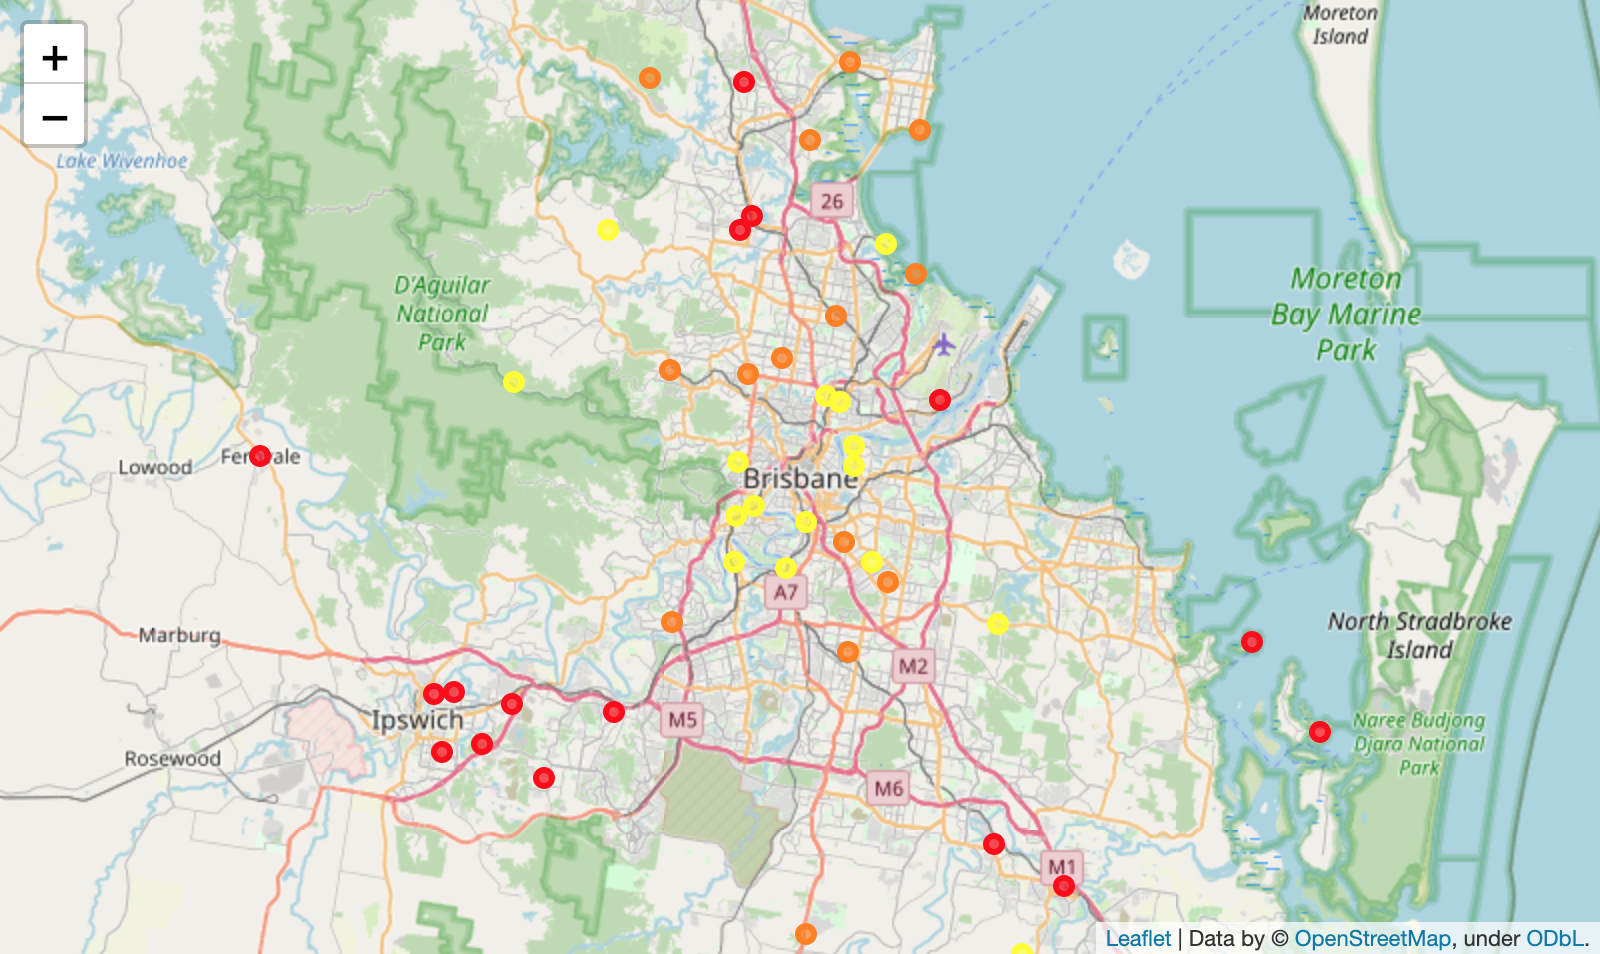
\includegraphics[width=0.49\textwidth,keepaspectratio]{Figures/BrisbanePrices}}
            \subfigure[]{\label{Fig:MelbournePrices}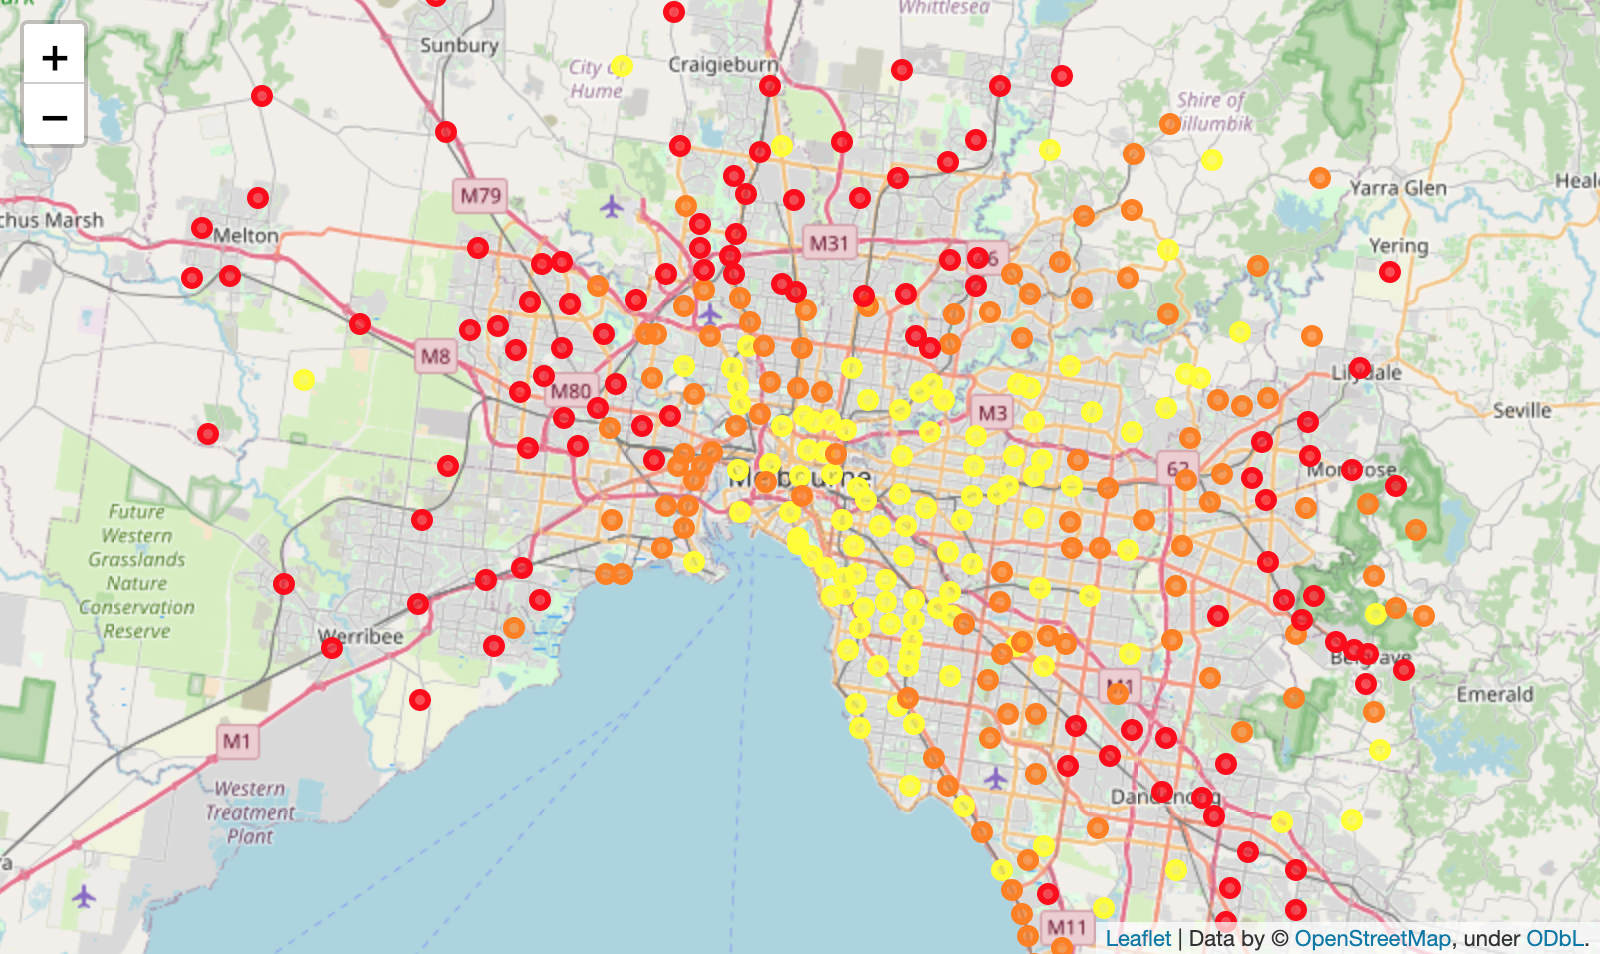
\includegraphics[width=0.49\textwidth,keepaspectratio]{Figures/MelbournePrices}} \\
            \subfigure[]{\label{Fig:SydneyPrices}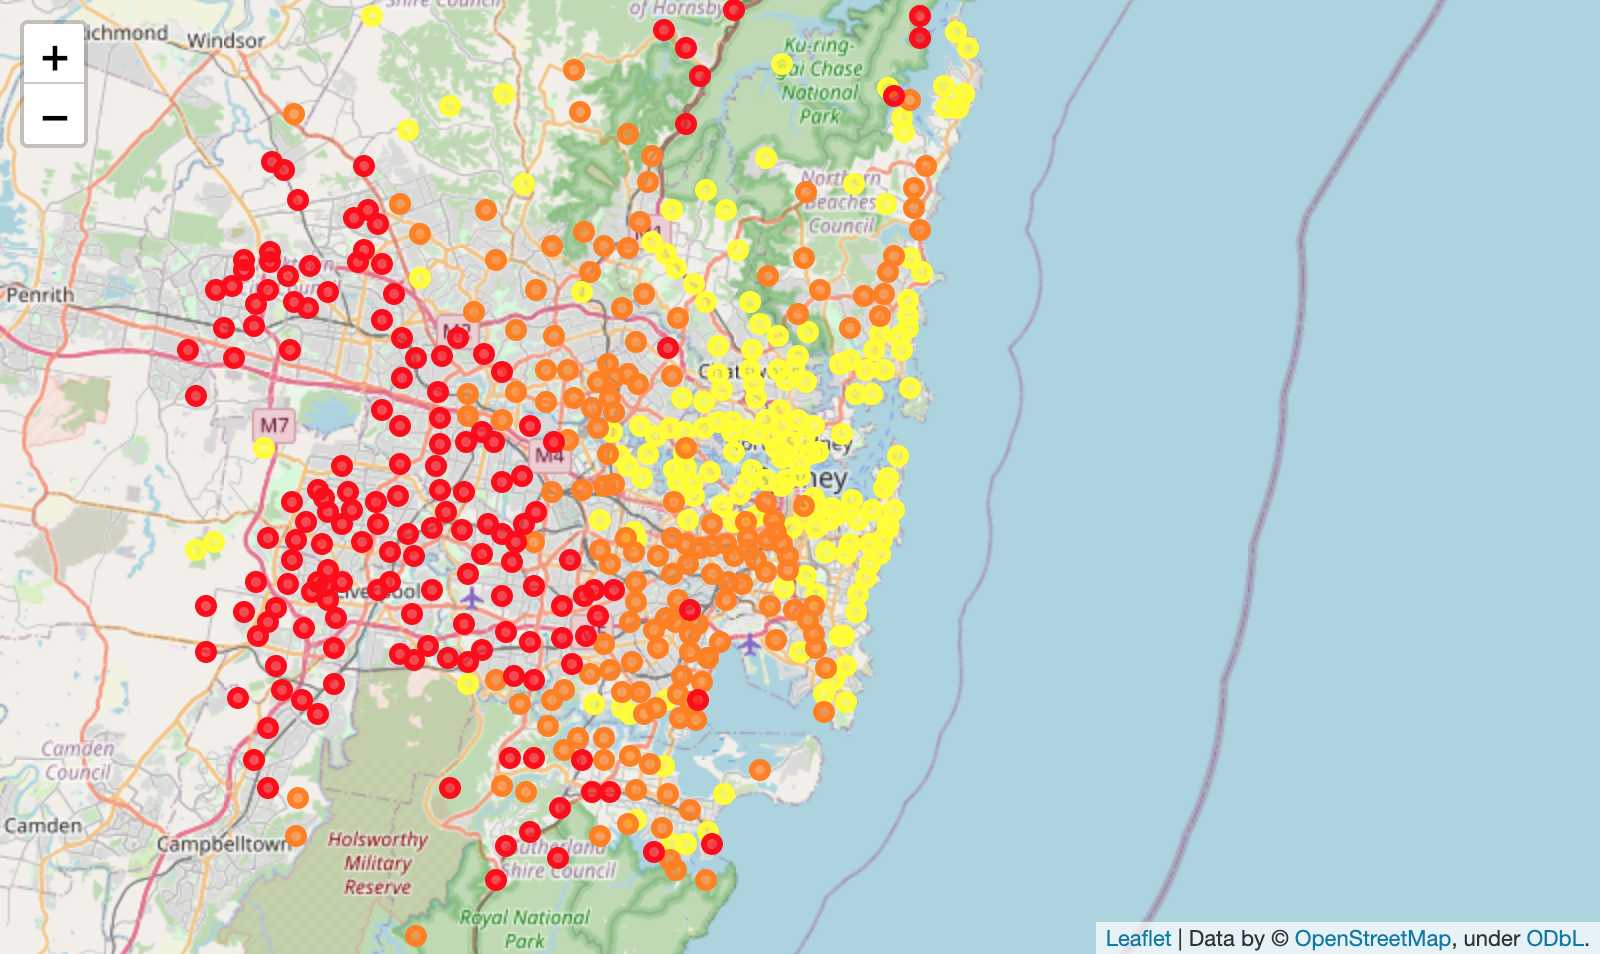
\includegraphics[width=0.49\textwidth,keepaspectratio]{Figures/SydneyPrices}}
            \subfigure[]{\label{Fig:PerthPrices}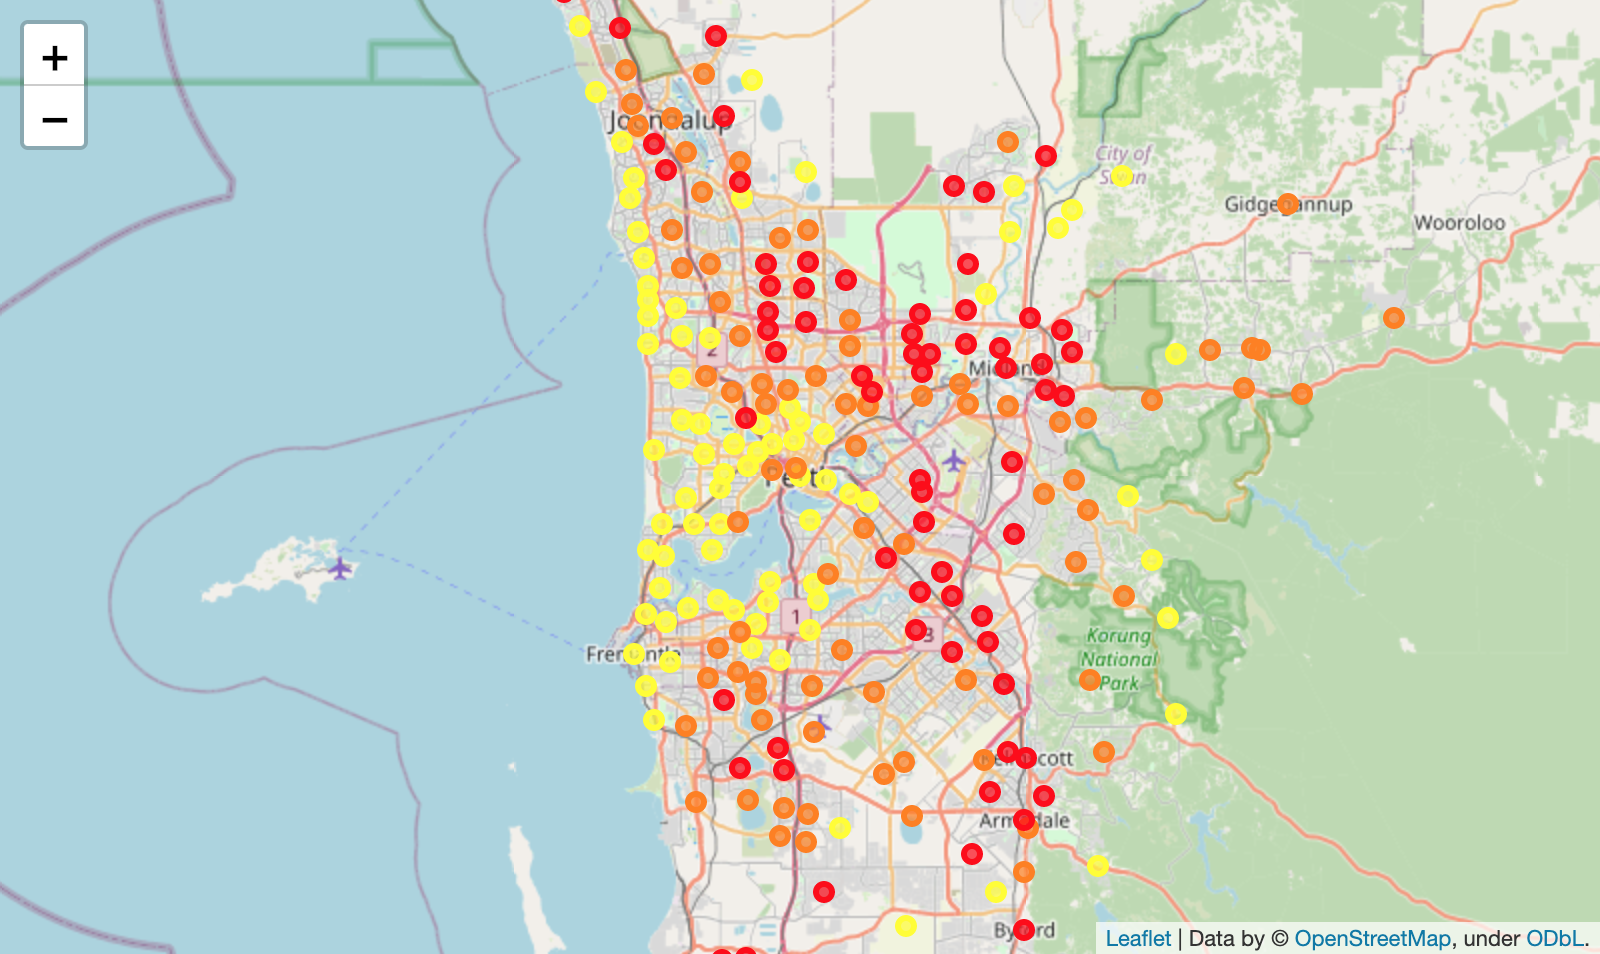
\includegraphics[width=0.49\textwidth,keepaspectratio]{Figures/PerthPrices}} \\
        \end{center}
        \caption{City suburb prices grouped into 3 bins (a) Brisbane (b) Melbourne (c) Sydney (d) Perth. Note that with the `autumn' colourmap used, yellow markers indicate the highest prices and red indicate the lowest prices.}
    \end{figure}

    Figures \ref{Fig:BrisbanePrices}-\ref{Fig:PerthPrices} present Leaflet maps generated with the \emph{Folium} library, using markers to locate and colour the suburbs by price. For each city the suburb median house prices were grouped into three bins using the \emph{Pandas} `qcut' function. Furthermore, for comparison with the distance to the CBD, Figures \ref{Fig:BrisbaneDistanceToCBD}-\ref{Fig:PerthDistanceToCBD} present the same Leaflet maps, but colouring the markers by the distance to the CBD. One observation that can be made is that, as one would intuitively believe, the most expensive suburbs tend to be those that are in close proximity to the CBD with a gradual and almost radial reduction in price as one moves further away from the CBD. An interesting exception here is with Sydney and Perth, which are located near a long coastline. In these cases the house prices remain high along the coast, even as the distance to the CBD increases. Suburbs that spread inland however, tend to show the more expected decrease in house price with increasing distance from the CBD.

    % Folium visualisation of suburb distance to CBD
    \begin{figure}[h!]
        \begin{center}
            \subfigure[]{\label{Fig:BrisbaneDistanceToCBD}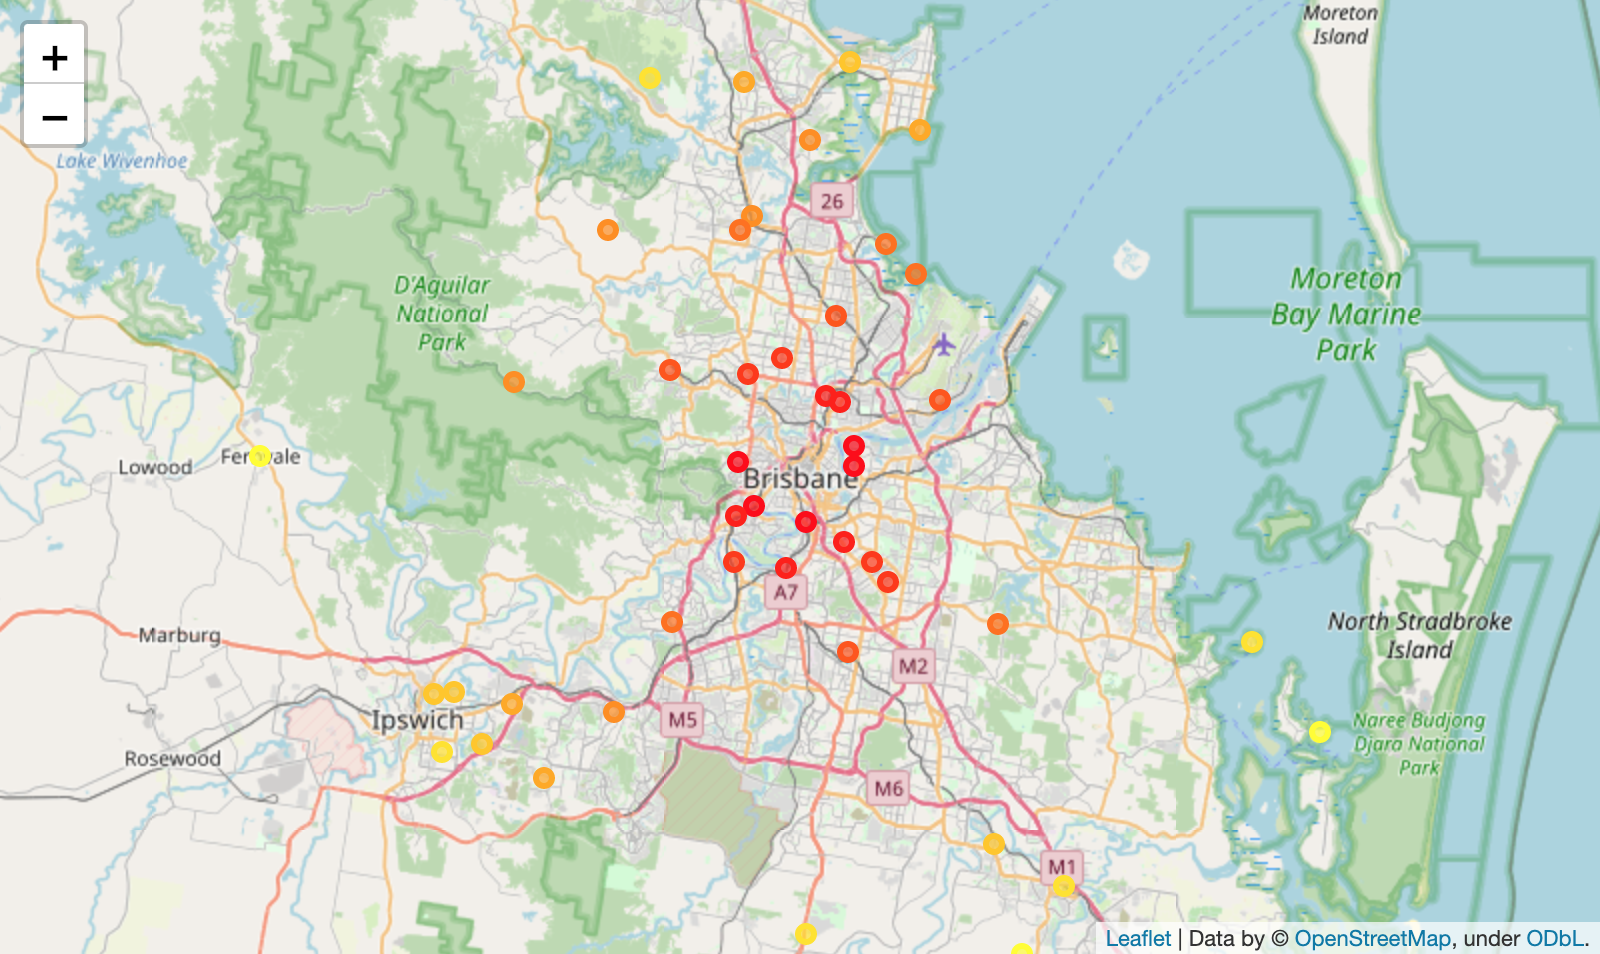
\includegraphics[width=0.49\textwidth,keepaspectratio]{Figures/BrisbaneDistanceToCBD}}
            \subfigure[]{\label{Fig:MelbourneDistanceToCBD}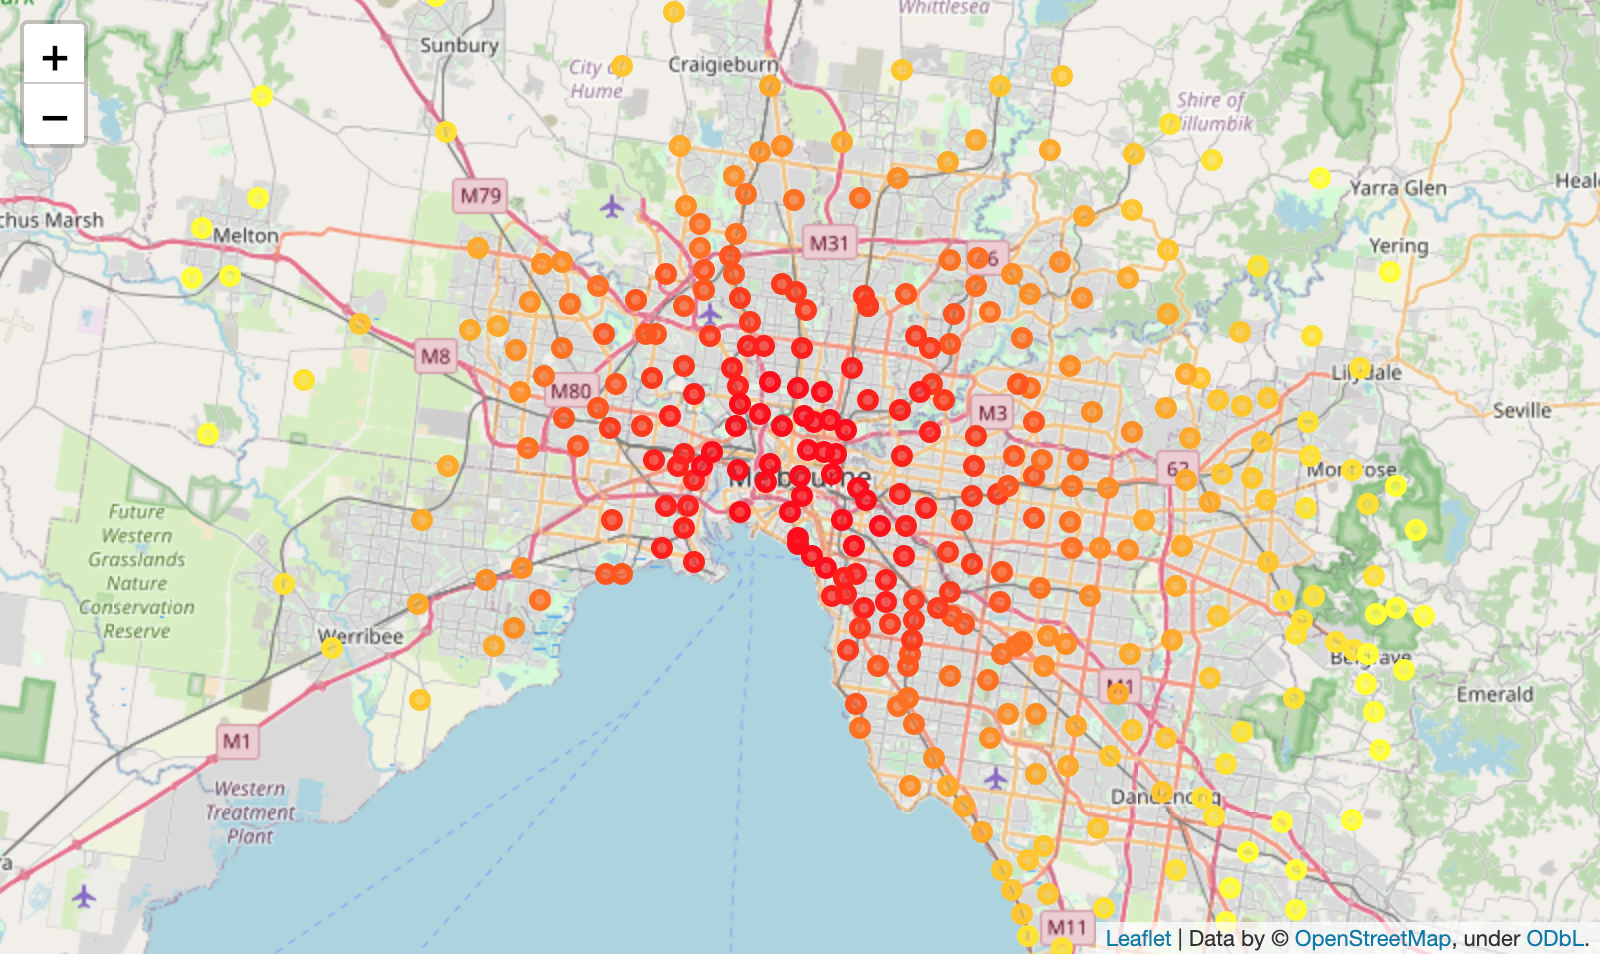
\includegraphics[width=0.49\textwidth,keepaspectratio]{Figures/MelbourneDistanceToCBD}} \\
            \subfigure[]{\label{Fig:SydneyDistanceToCBD}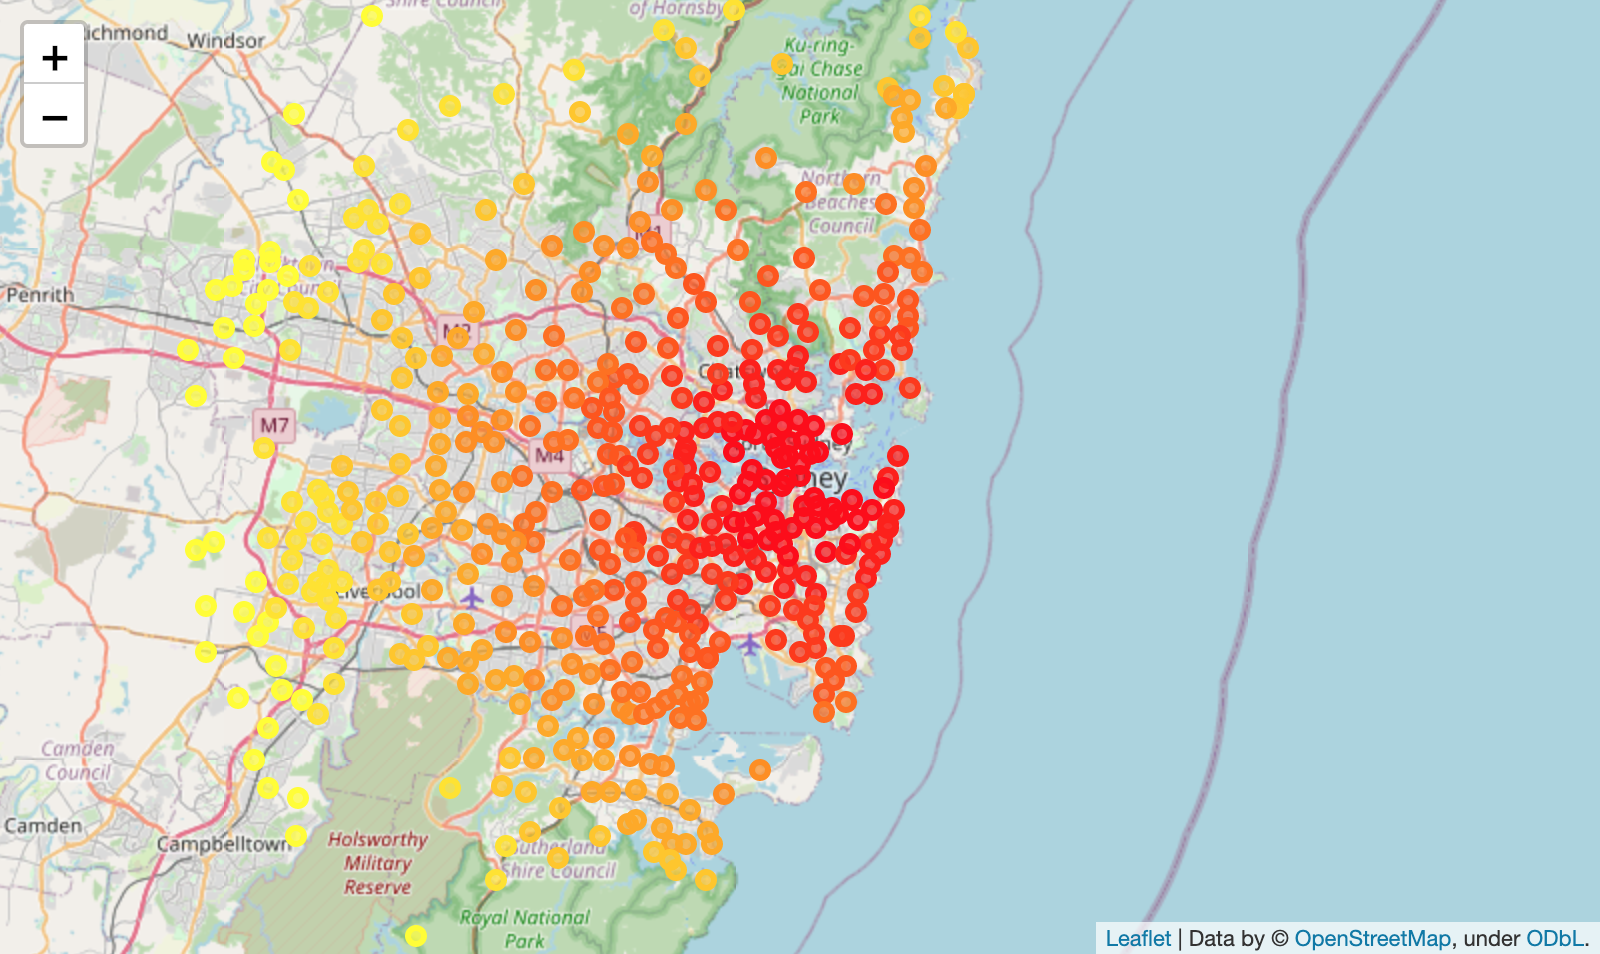
\includegraphics[width=0.49\textwidth,keepaspectratio]{Figures/SydneyDistanceToCBD}}
            \subfigure[]{\label{Fig:PerthDistanceToCBD}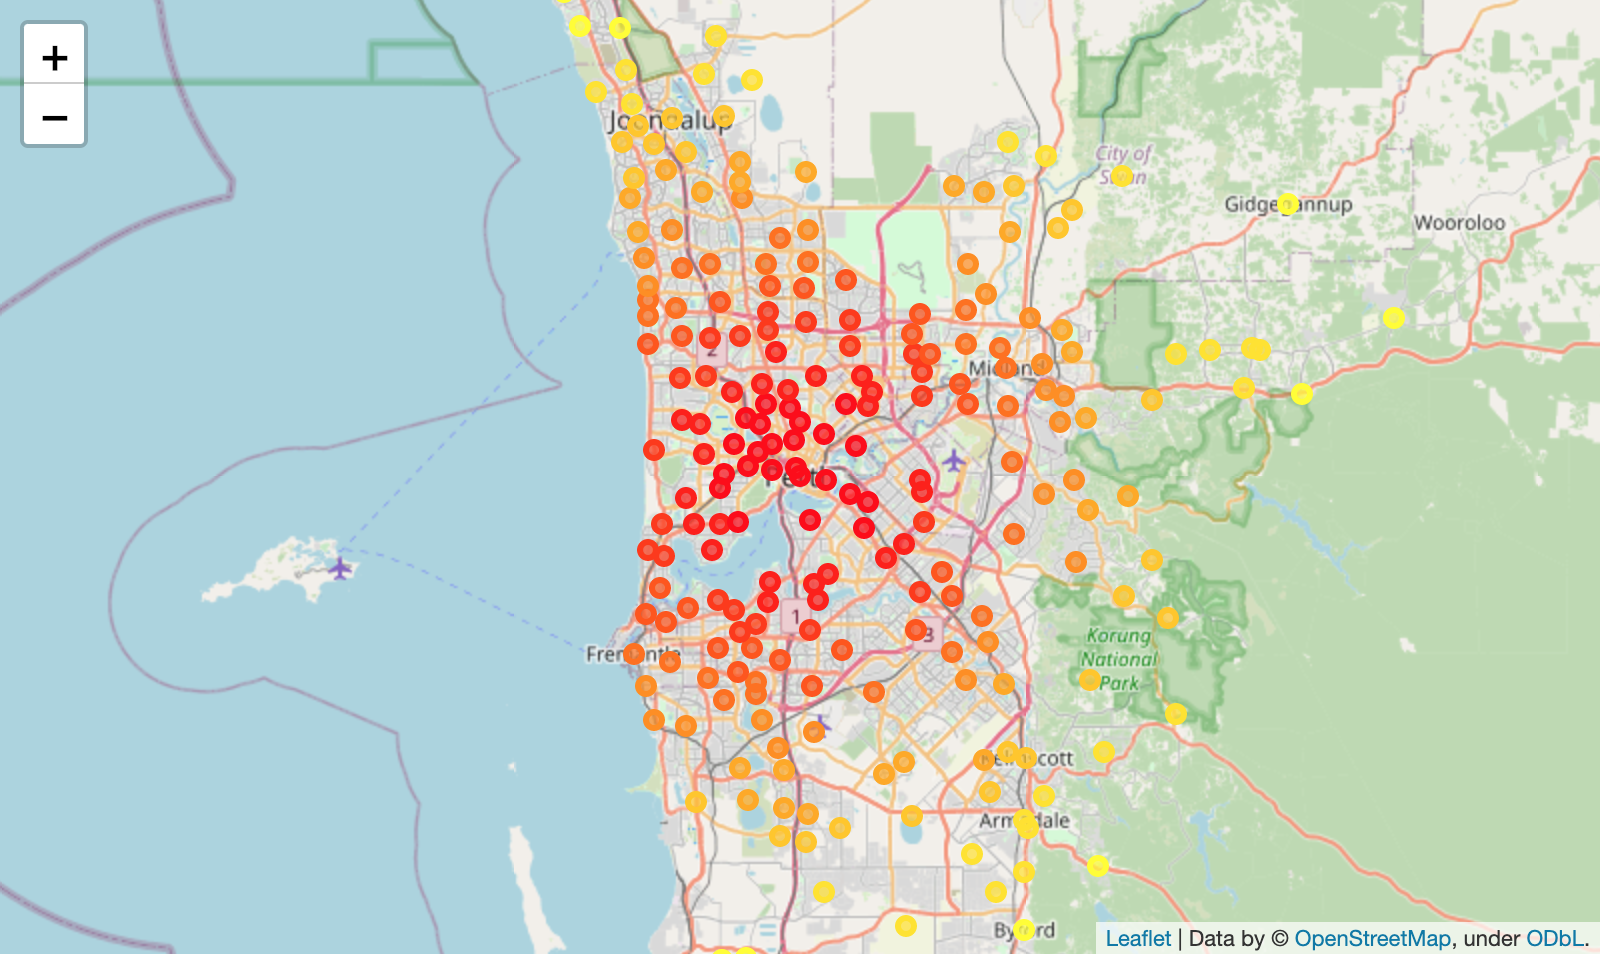
\includegraphics[width=0.49\textwidth,keepaspectratio]{Figures/PerthDistanceToCBD}} \\
        \end{center}
        \caption{City suburb distances to CBD grouped into 10 bins (a) Brisbane (b) Melbourne (c) Sydney (d) Perth. Note that with the `autumn' colourmap used, yellow markers indicate the suburbs furthest from the CBD and red indicate the closest suburbs to the CBD.}
    \end{figure}

    \clearpage

    Using the data frame containing nearby values for each suburb, Figures \ref{Fig:BrisbaneMostCommonVenues}-\ref{Fig:PerthMostCommonVenues} present the top ten most common venues for the two most expensive and two least expensive suburb for each city. One interesting observation that can be made is that the most common venues tend to include cafes, supermarkets, convenience/liquor stores, various restaurants, parks, gyms, and sports clubs. One perhaps unexpected result is that there does not appear to be any obvious difference in the most common venues when considering the most expensive or least expensive suburbs, hinting at the likelihood that predicting the house price for a suburb, based on the nearby venues is unlikely to be successful.

    % Most common venues
    \begin{figure}[h!]
        \begin{center}
            \subfigure[]{\label{Fig:BrisbaneMostCommonVenues}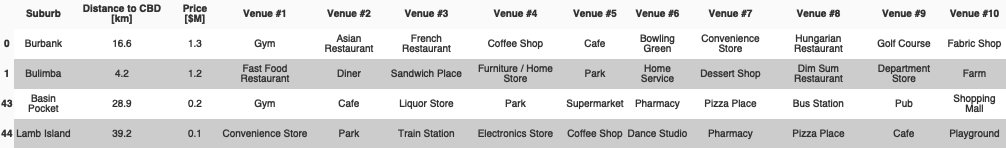
\includegraphics[width=0.99\textwidth,keepaspectratio]{Figures/BrisbaneMostCommonVenues}} \\
            \subfigure[]{\label{Fig:MelbourneMostCommonVenues}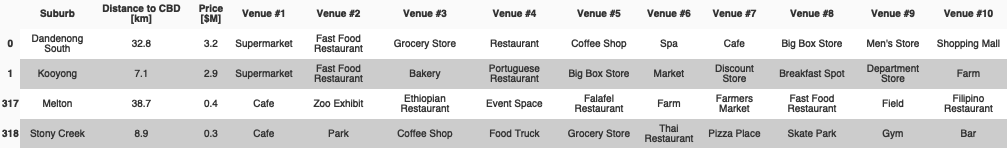
\includegraphics[width=0.99\textwidth,keepaspectratio]{Figures/MelbourneMostCommonVenues}} \\
            \subfigure[]{\label{Fig:SydneyMostCommonVenues}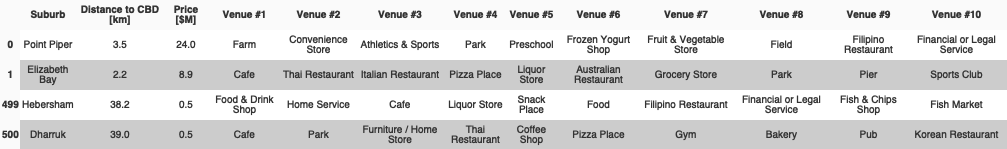
\includegraphics[width=0.99\textwidth,keepaspectratio]{Figures/SydneyMostCommonVenues}} \\
            \subfigure[]{\label{Fig:PerthMostCommonVenues}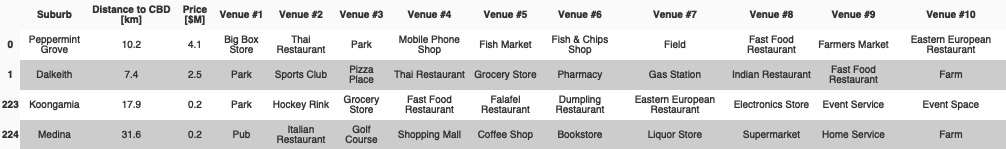
\includegraphics[width=0.99\textwidth,keepaspectratio]{Figures/PerthMostCommonVenues}}
        \end{center}
        \caption{The top ten most common venues in the two most expensive and two least expensive suburbs in (a) Brisbane (b) Melbourne (c) Sydney (d) Perth.}
    \end{figure}

    \clearpage

    In order to perform the k-means clustering, the optimal number of clusters for each city was obtained by using the `KElbowVisualizer' from the \emph{yellowbrick} library. Figure \ref{Fig:PerthDistortionScoreElbow} presents an example result for the city of Perth, illustrating that the elbow is located at ten clusters and hence, this was the the number used for the k-means analysis. The same approach was used for the other cities using 14 clusters for Brisbane, 14 clusters for Melbourne, and 18 clusters for Sydney.

    % Elbow score
    \begin{figure}[h!]
        \begin{center}
            \label{Fig:PerthDistortionScoreElbow}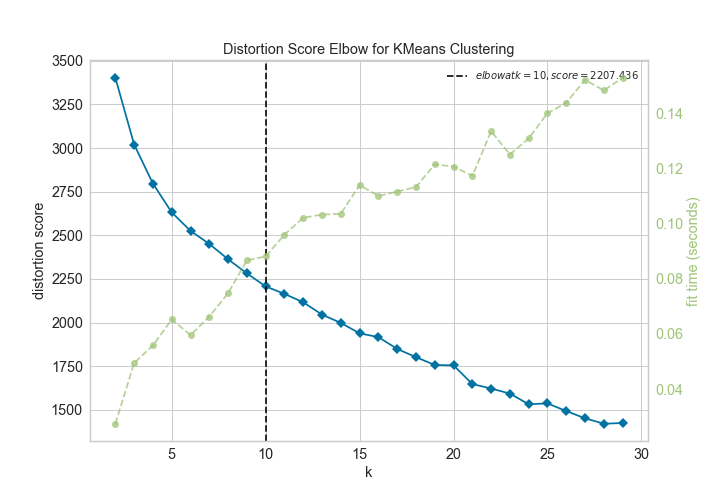
\includegraphics[width=0.49\textwidth,keepaspectratio]{Figures/PerthDistortionScoreElbow}
        \end{center}
        \caption{An example plot of the distortion score used to find the elbow and hence the optimal number of clusters for the city of Perth.}
    \end{figure}

    Figures \ref{Fig:BrisbaneClusters}-\ref{Fig:PerthClusters} present Leaflet maps for the four cities, using markers to locate and colour the suburbs by the resulting k-means assigned cluster label. As can be observed, there is no discernible pattern in terms of the locations of the clusters, with different clusters being scattered almost randomly throughout the city. The only exception to this trend is with Melbourne, where some unique clusters are found on the coast to the south west.

    % Folium visualisation of suburb clusters
    \begin{figure}[h!]
        \begin{center}
            \subfigure[]{\label{Fig:BrisbaneClusters}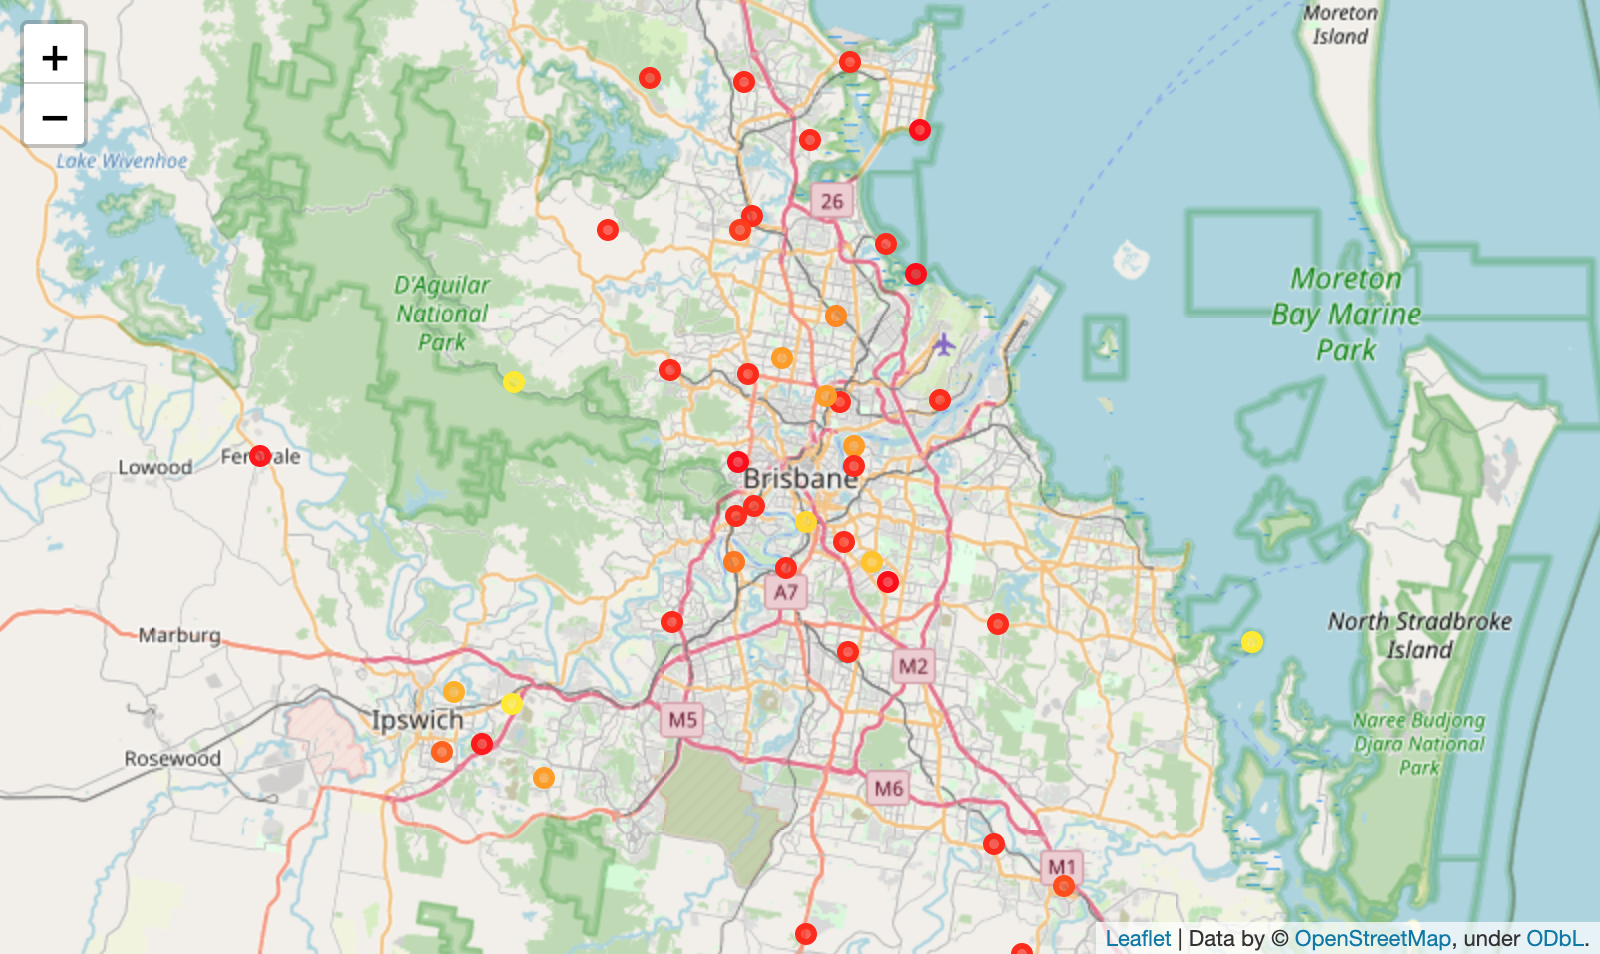
\includegraphics[width=0.49\textwidth,keepaspectratio]{Figures/BrisbaneClusters}}
            \subfigure[]{\label{Fig:MelbourneClusters}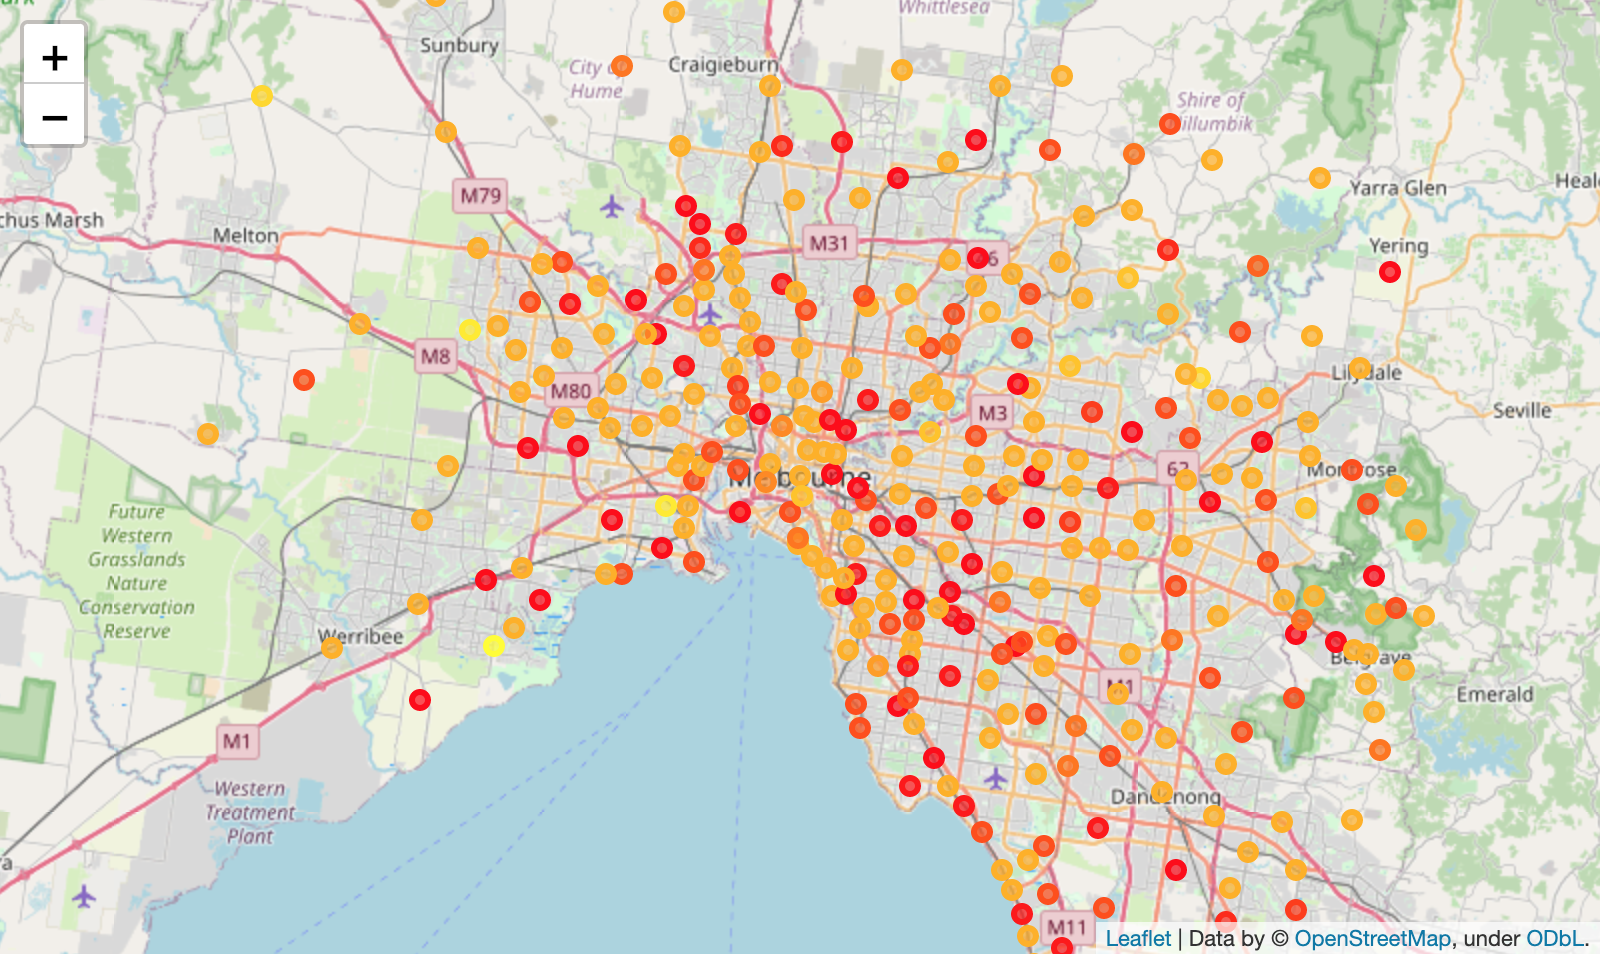
\includegraphics[width=0.49\textwidth,keepaspectratio]{Figures/MelbourneClusters}} \\
            \subfigure[]{\label{Fig:SydneyClusters}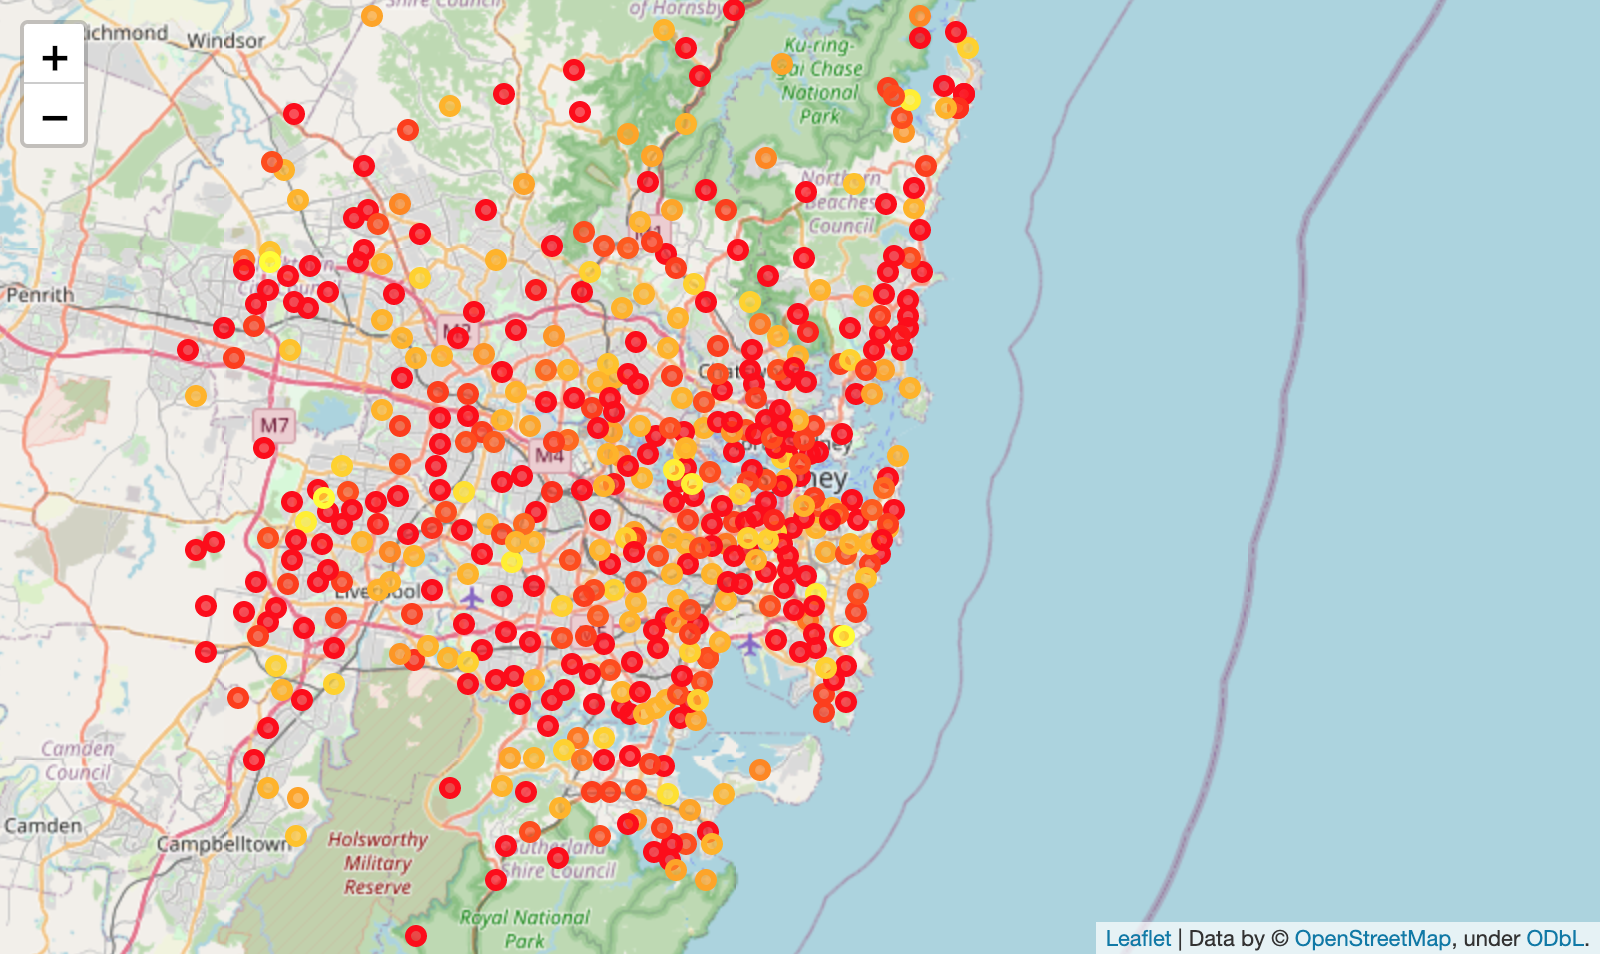
\includegraphics[width=0.49\textwidth,keepaspectratio]{Figures/SydneyClusters}}
            \subfigure[]{\label{Fig:PerthClusters}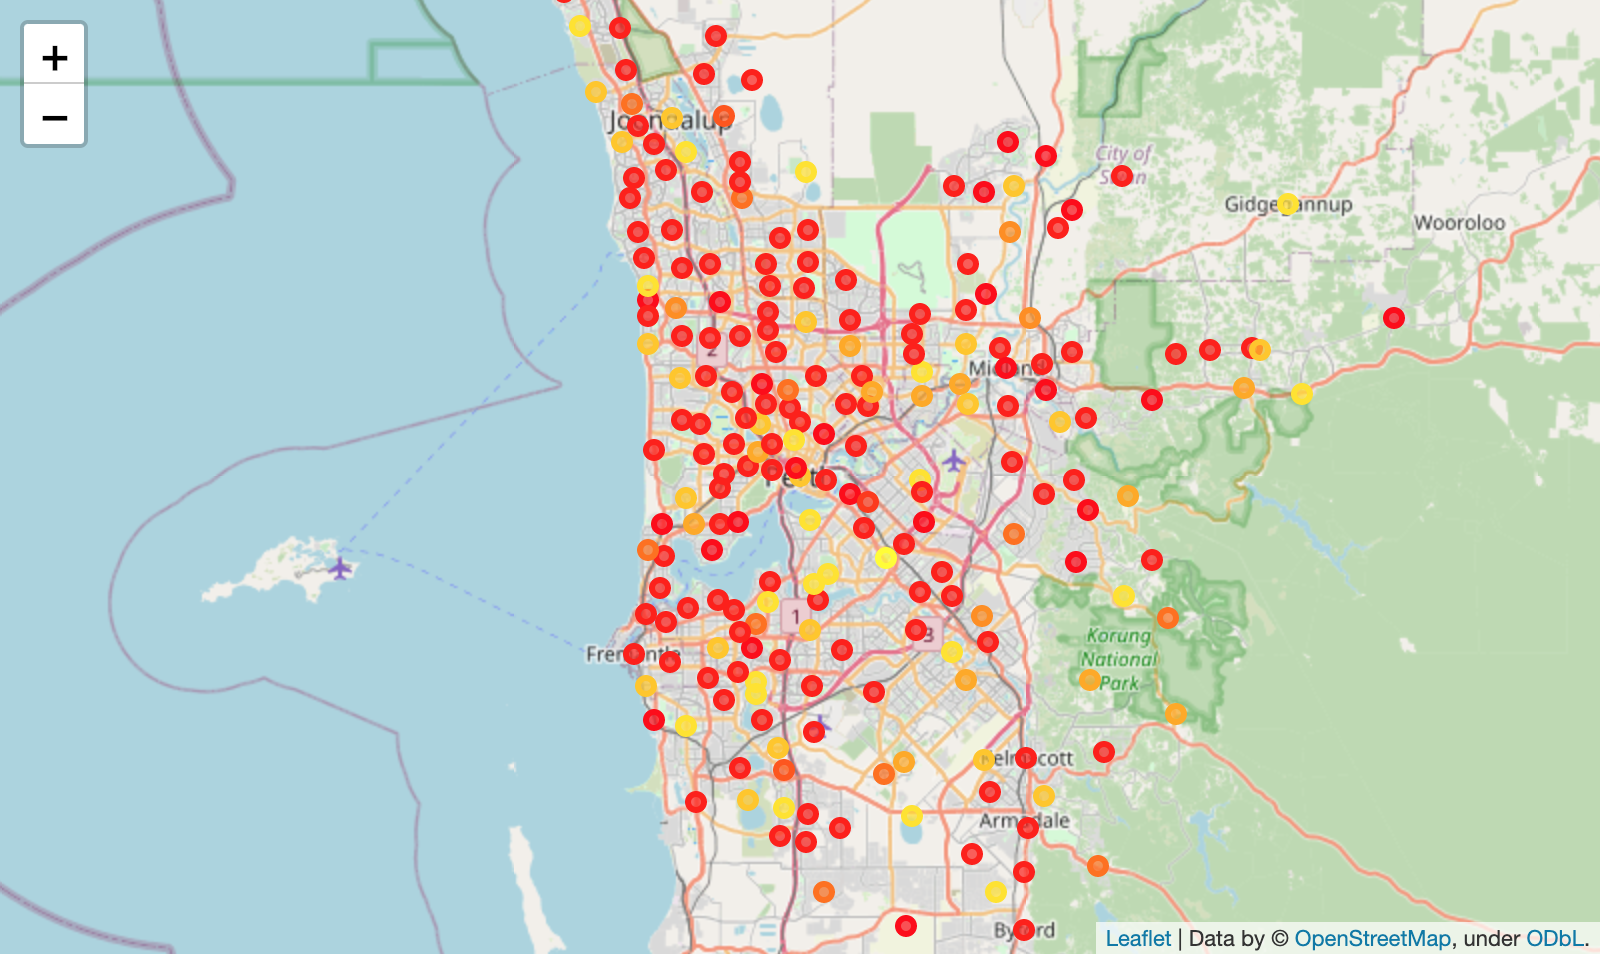
\includegraphics[width=0.49\textwidth,keepaspectratio]{Figures/PerthClusters}}
        \end{center}
        \caption{City suburb distances to CBD grouped into 10 bins (a) Brisbane (b) Melbourne (c) Sydney (d) Perth.}
    \end{figure}

    \clearpage

    % City suburb prices vs distance to CBD and second order polynomial fit
    \begin{figure}[h!]
        \begin{center}
            \subfigure[]{\label{Fig:BrisbanePriceVsDistanceToCBD}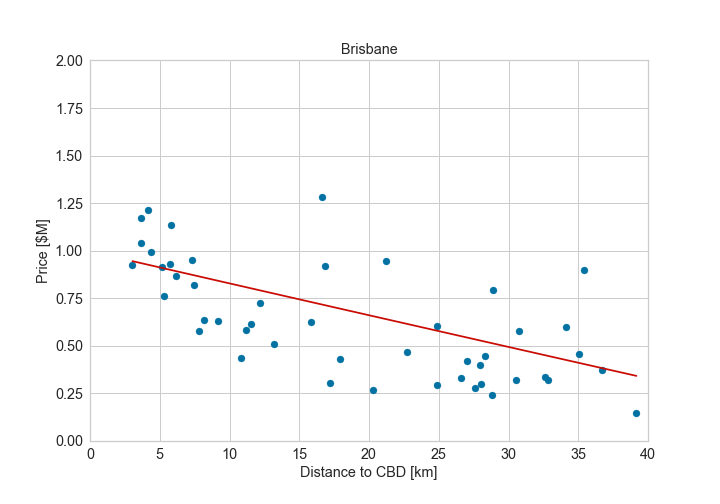
\includegraphics[width=0.49\textwidth,keepaspectratio]{Figures/BrisbanePriceVsDistanceToCBD}}
            \subfigure[]{\label{Fig:MelbournePriceVsDistanceToCBD}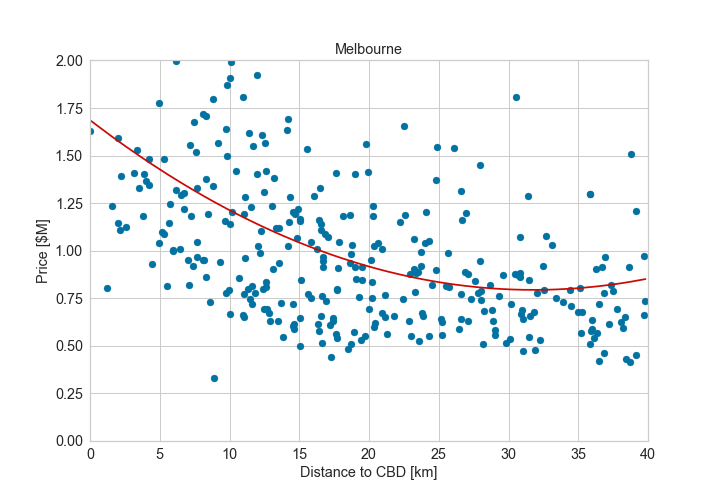
\includegraphics[width=0.49\textwidth,keepaspectratio]{Figures/MelbournePriceVsDistanceToCBD}} \\
            \subfigure[]{\label{Fig:SydneyPriceVsDistanceToCBD}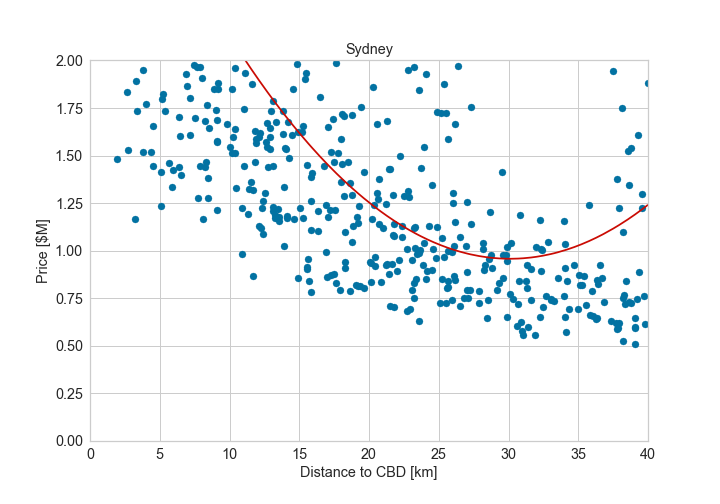
\includegraphics[width=0.49\textwidth,keepaspectratio]{Figures/SydneyPriceVsDistanceToCBD}}
            \subfigure[]{\label{Fig:PerthPriceVsDistanceToCBD}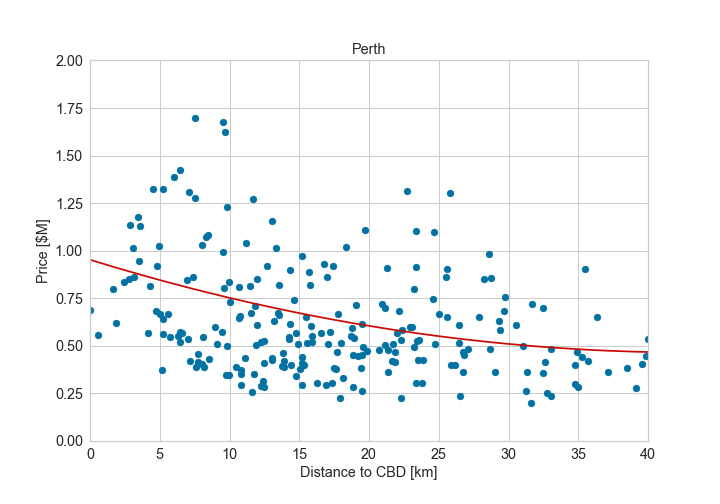
\includegraphics[width=0.49\textwidth,keepaspectratio]{Figures/PerthPriceVsDistanceToCBD}} \\
        \end{center}
        \caption{Scatter plots of suburb prices with a second order polynomial fit (a) Brisbane (b) Melbourne (c) Sydney (d) Perth.}
    \end{figure}

    In order to test the hypothesis that the distance to the CBD could be used to predict the median house price of a suburb, a simple polynomial regression analysis was performed for each city. Figures \ref{Fig:BrisbanePriceVsDistanceToCBD}-\ref{Fig:PerthPriceVsDistanceToCBD} present scatter plots for each city, showing the resulting second order polynomial, fit with the `LinearRegression' model using `PolynomialFeatures' from the \emph{sklearn} library. As can be observed, while there is a lot of variance about the regression curves, there also appears to be a general second order decrease in house price with distance from the CBD, but for Melbourne and Sydney the prices increase again around the 40km cutoff value. When looking at the prices as depicted in the Leaflet maps of Figures \ref{Fig:BrisbanePrices}-\ref{Fig:PerthPrices} it can be observed that there are in fact a number of expensive suburbs far away from the CBD more rural areas, in an almost radial pattern. This result is partly a consequence of the 40km cutoff and if it had been reduced to around 30km or so, this effect would most likely not have been observed.

    % Mean Squared Errors
    \begin{table}[h!]
        \centering
        \begin{tabular}{|c|c|c|}
            \hline
            \textbf{City}   & \textbf{Suburb Distance to CBD [km]}   & \textbf{Suburb Nearby Venues} \\
                            & \textbf{$2^{nd}$ Order Polynomial MSE} & \textbf{SVR MSE} \\
            \hline
            Brisbane    & 0.1051                         & 0.0973 \\
            Melbourne   & 0.0626                         & 0.2570 \\
            Sydney      & 1.0823                         & 1.0243 \\
            Perth       & 0.1005                         & 0.2720 \\

            \hline
        \end{tabular}
        \label{Tab:CityMSEs}
        \caption{Comparison of the mean squared errors (MSE) for two different approaches to predicting a suburb's median house price.}
    \end{table}

    Finally, in order to test the hypothesis that a suburb's nearby venues could be used as a means to predict the median house price, a support vector regressor (SVR) from the \emph{sklearn} library was used with the suburb's one hot encoded set of nearby venues. Although it would seem unlikely that this approach would be successful, given the almost random clustering of suburbs, an extensive sweep over the SVR parameters was performed with the `GridSearchCV class' using a five fold cross validation, to obtain the optimal hyper-parameters. The parameters swept over the `kernel', testing linear, polynomial, and radial basis functions (and for the polynomial kernel swept over polynomial degrees 1-6), and swept over a regularisation parameter in the range of $10^{-6}-1$. For all cities, the polynomial kernel produced the best score, with degrees 5 for Brisbane and Melbourne, degrees 2 for Sydney, and degree 1 for Perth. The best regularisation parameters were in the range of $10^{-4}-10^{-3}$. Once the optimal hyper-parameters for each city had been found, the SVR was finally retrained on 70\% of the suburb data with the mean squared error (MSE) computed based on the remaining 30\%. Table \ref{Tab:CityMSEs} presents a comparison of the mean squared errors for the two approaches. As can be observed, the second order polynomial regression using a suburb's distance to the CBD tended to produce the lowest MSEs. Surprisingly however, the SVR produced MSEs that were in a similar range (at least for Brisbane and Sydney). As a final test the SVR was retrained using \emph{both} the distance to the CBD and nearby venues as features using the same grid search approach, but the MSEs showed only a minor improvement over using just the nearby venues and are hence not presented.

\section{Discussion}

    The analyses performed on the median house prices of each suburb of Brisbane, Melbourne, Sydney, and Perth show that in general, the price follows a quadratic decrease with distance from the CBD. This is intuitively what one might expect, but also useful to see this effect presented in a quantitative manner. When comparing the four cities it is apparent that Sydney has the broadest distribution in house price, with many expensive suburbs having median house prices well over \$1 million. When comparing nearby venues, it is apparent that both the most expensive and least expensive suburbs appear to contain similar venues such as cafes, supermarkets, parks, and sports venues. It is interesting to note that for cities like Melbourne, where a suburb's median house price correlates reasonably well with distance to the CBD, the polynomial regressor using this feature performed significantly better than the SVR using the suburbs nearby venues. For cities like Sydney where expensive suburbs along the coast violate this trend, using the nearby venues proves as useful a predictor as the nearby venues. Perhaps a more detailed analysis of the individual suburbs focussing on specific venues such as beaches, highly ranked schools, or proximity to public transport, or conversely industrial areas, airports, etc, might result in a clearer separation between the expensive suburbs, but this remains future work.  

\section{Conclusion}

    This report performed an analysis of the median house prices of four major Australian cities, assembling a dataset of location, price, proximity to the CBD, and nearby venues. The analysis included Leaflet maps visualising the suburbs and their prices, performed both clustering and regression in an attempt to see if the types of nearby venues correlate with the median house price, or could be used to predict the median house price. The results indicated that both the most and least expensive suburbs are comprised of similar venues and that while the proximity to the CBD serves as a `reasonable' feature with which to predict the house price, the types of venues do not. A more detailed analysis is likely required in order to build a more predictive model of a suburbs median house price.

\end{document}
